\documentclass[professionalfonts, aspectratio=169]{beamer}  
\usefonttheme{serif}                                        % Font theme: serif
\usepackage[utf8]{inputenc}                                 % Allows the use of different input encodings
\usepackage{graphicx}                                       % Enhanced support for graphics
\usepackage{amsmath}                                        % Enhances the typesetting of mathematics
\usepackage{amsfonts}                                       % Extra mathematical fonts
\usepackage{amssymb}                                        % Extra mathematical symbols
\usepackage{threeparttable}                 % For table notes
\usepackage{tikz}
\usetikzlibrary{shapes,arrows,positioning}
\usepackage{booktabs}                                       % Enhances the quality of tables
\usepackage{pgfplots}
\pgfplotsset{compat=1.17}
\usepackage{multirow}
% link settings
\usepackage{hyperref}                       % For hyperlinks
\usepackage[authoryear]{natbib}             % For bibliography

\usepackage{appendixnumberbeamer} % Numbering appendixes in beamer
\pdfstringdefDisableCommands{
  \def\translate{}
}
\usepackage{dcolumn}
\setbeamertemplate{navigation symbols}{} % Remove navigation symbols
\setbeamertemplate{footline}[frame number] % Add page number

% \setbeamercovered{transparent}  % Semi-transparent overlay

%---- Set the title page ----%
\title{Risk Adjustment, Self-Selection and Plan Design \\ in Medicare Advantage}
\institute{Stony Brook University}
\author{Zhu Liang}
\date{\today}

%---- Begin the document ----%
\begin{document}

\AtBeginSection[] % At the beginning of each section...
{
  \begin{frame}[noframenumbering, plain] % Create a new frame without a frame number
    \tableofcontents[currentsection] % Display the table of contents for the current section
  \end{frame}
}

\begin{frame}[noframenumbering, plain] % title frame without a frame number
    \titlepage
\end{frame}

%---- The slides structure ----%
\section{Introduction}

\begin{frame}{Medicare System}
  Medicare is a U.S. federal health insurance program mainly for individuals aged 65 and older, comprising two main components:
  \begin{itemize}
    \item \textbf{Traditional Medicare (TM)}: Usually combined with Medigap plans, offering generous coverage but higher premiums.
    \item \textbf{Medicare Advantage (MA)}: A managed competition system where the government subsidizes private insurers to provide plans with lower premiums and reduced coverage.
  \end{itemize}
\end{frame}

\begin{frame}{Medicare Advantage}
  \begin{itemize}
    \item \textbf{Managed Competition}: The government provides fixed and predetermined subsidies to private insurance firms, which in turn offer insurance plans to beneficiaries.
    \item \textbf{Cream Skimming}: Firms strategically target healthier beneficiaries to maximize profits.
    \item \textbf{Risk Adjustment}: The government adjusts subsidy payments to insurers based on beneficiaries' observable characteristics.
    \item Can risk adjustment effectively neutralize insurers' incentives for cream skimming when beneficiaries have private information about their health status?
  \end{itemize}
\end{frame}

\begin{frame}{Simplified Risk Adjustment Scenario}
  \begin{itemize}
    \item Equal numbers of young and old individuals:
    \begin{itemize}
      \item \textbf{Young}: 80\% healthy, 20\% sick
      \item \textbf{Old}: 20\% healthy, 80\% sick
    \end{itemize}
    \item Cost of care: \$1,000 for healthy individuals, \$5,000 for sick individuals
    \item Age is observable to the government; health status is private information \pause
    \item Subsidy risk-adjusted by age:
    \begin{itemize}
      \item \textbf{Young}: \$1,000 $\times$ 0.8 + \$5,000 $\times$ 0.2 = \$1,800
      \item \textbf{Old}: \$1,000 $\times$ 0.2 + \$5,000 $\times$ 0.8 = \$4,200
    \end{itemize}
    \item Average subsidy rate by health status:
    \begin{itemize}
      \item \textbf{Healthy}: \$1,800 $\times$ 0.8 + \$4,200 $\times$ 0.2 = \$2,240\ (\textbf{above} cost of \$1,000)
      \item \textbf{Sick}: \$1,800 $\times$ 0.2 + \$4,200 $\times$ 0.8 = \$3,960\ (\textbf{below} cost of \$5,000)
    \end{itemize}
    \item \textbf{Firms still prefer healthy individuals even after risk adjustment}.
  \end{itemize}
\end{frame}

\begin{frame}{Self-Selection and Strategic Plan Design}
  \begin{itemize}
    \item When beneficiaries have private information about their health status, they can engage in self-selection when choosing plans.
    \item Firms can strategically design their plans to attract healthier individuals through this self-selection (e.g., lower premiums, less generous coverages).
  \end{itemize}
\end{frame}

\begin{frame}{Motivation}
  \begin{itemize}
    \item Medicare Advantage (MA) has gained popularity, with 54\% of Medicare beneficiaries enrolled in MA plans as of 2024.
    \item Previous studies indicate that competition in MA markets can enhance welfare but often neglect the impact of self-selection based on private information.
    \item Current risk adjustment mechanisms fail to account for self-selection and endogenous plan design, potentially causing market distortions.
  \end{itemize}
\end{frame}

\begin{frame}{Research Questions}
  \begin{itemize}
    \item How does self-selection influence plan design and market outcomes in MA market?
    \item What are the welfare implications of these interactions?
  \end{itemize}
\end{frame}

\begin{frame}{Methodology}
  \begin{itemize}
    \item Develop a structural model of demand and supply that incorporates self-selection and endogenous plan design.
    \item Estimate the model using Medicare Advantage data.
    \item Conduct counterfactual simulation to analyze scenario where self-selection effects are neutralized.
  \end{itemize}
\end{frame}

\begin{frame}{Key Findings}
  Counterfactual simulation indicate that if the risk adjustment policy can neutralize self-selection effect:
  \begin{itemize}
    \item Consumer surplus increases by 11\%
    \item Firm profits increase by 34.6\%
    \item No significant change in government spending
  \end{itemize}
\end{frame}

\begin{frame}{Contributions}
  \begin{itemize}
    \item \textbf{Theoretical}: Developed a managed competition model incorporating endogenous plan design and self-selection under private information.
    \item \textbf{Empirical}: Applied the model to Medicare Advantage data, evaluating the welfare implications of self-selection effects.
    \item \textbf{Policy}: Provided insights for enhancing risk adjustment payment policies to mitigate market distortions.
  \end{itemize}
\end{frame}

\section{Data}

\begin{frame}{Data}
  \begin{itemize}
    \item \textbf{Individual Level}: Medicare Current Beneficiary Survey (MCBS)
    \begin{itemize}
      \item Contains detailed information on individual beneficiaries, including demographics and plan choice.
    \end{itemize}
    \item \textbf{Plan Level}: Centers for Medicare and Medicaid Services (CMS) datasets on MA plans
    \begin{itemize}
      \item Includes data on plan generosity levels, premiums, and other attributes such as network and additional benefits.
    \end{itemize}
  \end{itemize}
\end{frame}

\begin{frame}{Summary Statistics}
  \begin{table}[ht]
  \scriptsize
  \renewcommand{\arraystretch}{1.2}
  \centering
  \begin{threeparttable}
    \caption{Consumer Summary Statistics by Plan Type}
    \begin{tabular}{ll|lll}
      \toprule
      \textbf{Category} & \textbf{Variable} & \textbf{TM} & \textbf{MA} & \textbf{Overall} \\
      \midrule
      \textbf{Demographics} & Age & 73.887 & 74.283 & 73.997 \\
      & Female & 0.524 & 0.557 & 0.533 \\
      & Income & 70,203 & 50,484 & 64,697 \\
      & White Race & 0.873 & 0.827 & 0.860 \\
      & Higher Education & 0.607 & 0.469 & 0.568 \\
      \textbf{Medicare} & Medical Spending & 8340 & 6012 & 7692 \\
      \bottomrule
    \end{tabular}
    \begin{tablenotes}
      \footnotesize
      \item Note: TM refers to Traditional Medicare, and MA refers to Medicare Advantage. Values are means for continuous variables and proportions for binary variables.
    \end{tablenotes}
  \end{threeparttable}
  \label{tab:consumer_summary}
\end{table}

\end{frame}
  


\section{Model}
\begin{frame}{Timing}
  \begin{itemize}
    \item \textbf{Government Sets Subsidy Rates:} Determines capitation payments using a risk adjustment formula.
    \item \textbf{Stage 1 - Firm Decisions:} Firms set the prices and generosity levels of their plans to maximize profit after accounting for subsidies.
    \item \textbf{Stage 2 - Consumer Choices:} Consumers choose plans (including the outside option) that best meet their needs, using their private information.
  \end{itemize}
\end{frame}

\begin{frame}{Demand: Private Information}
  Each consumer is characterized by two variables:
  \begin{itemize}
      \item An observable risk-adjusted capitation rate ($k_i$), which serves as a proxy for the average expected health expenditure within a cohort with similar observable characteristics.
      \item A private health perception ($\textcolor{red}{e_i}$), which directly influences their preference for plan generosity and, consequently, their plan choice.
  \end{itemize}

  \begin{equation}
    \ln(\textcolor{red}{e_i}) = \ln(k_i) + \tau_i, \quad \tau_i \sim N(0, \sigma_\tau^2)
  \end{equation}

\end{frame}

\begin{frame}{Demand: Utility}

  The utility of consumer $i$ from plan $j$ is given by

  \begin{equation}
    u_{ij} = \textcolor{red}{\beta_i} g_j - \alpha_i p_j + \lambda^{A}_i A_j + \lambda^X X_j + \xi_j + \varepsilon_{ij}.
  \end{equation}

  \begin{itemize}\small
    \item $g_j$ and $p_j$ are the generosity \footnote{Generosity is measured by expected OOP under a specific health condition} and premium of plan $j$.
    \item $A_j$ is MA type indicator
    \item $X_j$ is a vector of other plan characteristics
    \item $\xi_j$ is the unobserved plan-specific quality
    \item $\varepsilon_{ij}$ is the idiosyncratic error term, following a T1EV distribution
  \end{itemize}

  The utilitiy of the outside option (TM + Medigap) is
  \begin{equation}
    u_{i0} = \textcolor{red}{\beta_i} g_0 - \alpha_i p_0 + \xi_0 + \varepsilon_{i0}.
  \end{equation}
\end{frame}

\begin{frame}{Demand: Hetereogeneity}

  Preferences for plan generosity ($\textcolor{red}{\beta_i}$) are influenced by health perception $\textcolor{red}{e_i}$
  \begin{equation}
      \textcolor{red}{\beta_i} = \bar{\beta} + \gamma \ln \textcolor{red}{e_i}.
  \end{equation}
  Preferences for plan premiums ($\alpha_i$) are associated with income level
  \begin{equation}
      \alpha_i = \bar{\alpha} + \rho^{\text{inc}} \text{inc}_i.
  \end{equation}
  Preferences for the MA type ($\lambda^{A}_i$) relate to demographic factors and existing health coverage, including Medicaid eligibility and employer-sponsored insurance (ESI) coverage
  \begin{equation}
      \lambda^{A}_i = \bar{\lambda}^{A} + \rho^{\text{edu}} \text{edu}_i + \rho^{\text{white}} \text{white}_i + \rho^{\text{Mcd}} \text{Mcd}_i + \rho^{\text{ESI}} \text{ESI}_i.
  \end{equation}
  
\end{frame}

\begin{frame}{Demand: Plan Mean Utility}
  The mean utility of plan $j$ relative to the outside option is

  \begin{equation}
    \delta_j = \bar{\beta} (g_j - g_0) - \bar{\alpha} (p_j - p_0) + \bar{\lambda}^{A} A_j + \lambda^X X_j + \xi_j - \xi_0,
  \end{equation}
  and let the $\mu_ij$ denote the individual-specific deviation from $\delta_j$, we can rewrite the utility function as
  \begin{equation}
    u_{ij} = \delta_j + \mu_{ij} + \varepsilon_{ij}.
  \end{equation}

\end{frame}

\begin{frame}{Demand: Plan Choice Probability}
  Considering the T1EV distribution of $\varepsilon_{ij}$, the probability that consumer $i$ chooses plan $j$ is given by
  \begin{equation}
    s_{ij}(\textcolor{red}{e_i}) = 
    \frac{\exp \big(\delta_j + \mu_{ij}(\textcolor{red}{e_i}) \big)}
    {\sum_{j' = 0}^{J}  \exp \big(\delta_{j'} + \mu_{ij'}(\textcolor{red}{e_i}) \big)}.
  \end{equation}

  The market share of plan $j$ is given by the weighted sum of the individual choice probabilities
  \begin{equation}
    q_j = \sum_i w_i \cdot s_{ij}(\textcolor{red}{e_i}) = \sum_i w_i \cdot \int s_{ij}(e) \, dF_{e}(e).
\end{equation}
\begin{itemize}\small
  \item $w_i$ is the sampling weight of consumer $i$
\end{itemize}

\end{frame}

\begin{frame}{Supply: Competition Setting}
  \begin{itemize}
    \item \textbf{Bertrand-Nash Competition}: Firms compete on prices and plan generosity levels, considering plan offerings and other exogenous attributes, with each plan having specific cost functions.
    \item \textbf{Multi-Product, Multi-Market}: Firms operate as multi-product entities competing across multiple submarkets.
    \item \textbf{Short-Run Focus}: The model does not account for the entry and exit of plans.
    \item \textbf{Selection Effect}: The cost of plans is influenced not only by the plan's generosity level but also by the health status of the individuals who select the plan, which is itself affected by the plan's generosity.
  \end{itemize}
\end{frame}

\begin{frame}{Supply: Costs}

  The cost of a plan is influenced by its generosity level $g_j$ and other observable exogenous attributes $X_j$. The marginal cost function is expressed as:
  \begin{equation}
    \label{eq:marginal_cost}
    mc_j(g_j) = mc_j^g(g_j) + \underbrace{w^X \cdot X_j + \omega_j}_{\text{predetermined}},
  \end{equation}
  \begin{itemize}\small
    \item $\omega_j$ represents the unobserved plan-specific cost shock.
    \item Each plan has a unique cost function due to the predetermined components.
    \item Higher generosity in plans increases costs both directly, through more generous coverage, and indirectly, by attracting more sick individuals, which adds further expenses to the plan (the \textbf{Selection Effect}).
  \end{itemize}
\end{frame}

\begin{frame}{Supply: Plan Design Problem}
  The total profit for a firm in county $c$ is the aggregate of profits from all its offered plans
  \begin{equation}
      \pi_{f,c} = \sum_{j \in \mathcal{J}_{f,c}} \pi_{j}.
  \end{equation}

  The state-level profit for MA firm $f$ is then the sum of profits across all counties $c$ where firm $f$ operates
  \begin{equation}
      \pi_{f} = \sum_{c \in \mathcal{C}_f} \pi_{f,c},
  \end{equation}
  where $\mathcal{C}_f$ denotes the set of counties in which firm $f$ is active.

  The firm's plan design problem can be formulated as maximizing state-level profit by strategically setting bid and generosity levels for each plan
  \begin{equation}
  \label{eq:objective_function}
      \max_{b_f, g_f} \pi_{f} = \sum_{c \in \mathcal{C}_f } \sum_{j \in \mathcal{J}_{f,c} } (b_j - mc_j(g_j)) \cdot M_c \cdot s_{c,j}(g, b),
  \end{equation}

\end{frame}

\begin{frame}{Supply: Necessary Optimality Conditions}
  The first-order conditions for the firm's plan design problem are
  \begin{equation}
    \label{eq:bid_foc}
        \{b_j\}: \quad \sum_{c \in \mathcal{C}_f} 
        M_c \left(s_{c,j} + \sum_{j \in \mathcal{J}_{f,c}} (b_j - mc_j) \cdot \frac{\partial s_{c,j}}{\partial b_j} \cdot
        \frac{\partial b_j}{\partial p_j} \right) = 0 
        \quad \forall j,
    \end{equation}
    \begin{equation}
    \label{eq:generosity_foc}
        \{g_j\}: \quad \sum_{c \in \mathcal{C}_f} 
        M_c \left( 
            \frac{\partial mc_j}{\partial g_j} \cdot s_{c,j} - 
            \sum_{j \in \mathcal{J}_{f,c}}
            (b_j - mc_j) \cdot \frac{\partial s_{c,j}}{\partial g_j}
        \right) = 0
        \quad \forall j,
    \end{equation}
    where $\frac{\partial b_j}{\partial p_j} = 1$.

    Each firm faces unique optimization conditions due to differences in plan offerings and the specifics of their cost functions (see Equation \ref{eq:marginal_cost}).

\end{frame}

\section{Estimation}

\begin{frame}{Estimation: Consumer Heterogeneity}
  
\begin{table}[ht]\footnotesize
    \centering
    \caption{Estimation Results of Consumer Preference Heterogeneity}
    \label{tab:demand_result_1}
    \begin{tabular}{lccc}
        \toprule
        \textbf{Variable} & \textbf{Parameter} & \textbf{Estimate} & \textbf{Std Error} \\
        \midrule
        \textbf{Generosity Preference} & & & \\
        Health Perception & $\gamma$ & 0.115 & (0.052) \\
        \midrule
        \textbf{Premium Preference} & & & \\
        High Income Level & $\rho^{\text{inc}}$ & -0.473 & (0.248) \\
        \midrule
        \textbf{MA Type Preference} & & & \\
        High Education Level & $\rho^{\text{edu}}$ & -0.275 & (0.203) \\
        White Race & $\rho^{\text{white}}$ & -0.173 & (0.280) \\
        Medicaid Coverage & $\rho^{\text{Mcd}}$ & 0.039 & (0.244) \\
        ESI Coverage & $\rho^{\text{ESI}}$ & -2.543 & (0.404) \\
        \midrule
        \textbf{Private Information Distribution} & & & \\
        SD of Health Perception & $\sigma_{\tau}$ & 3.983 & (2.733) \\
        \bottomrule
    \end{tabular}
    \begin{threeparttable}
        \begin{tablenotes}\footnotesize
            \item \textit{Note}: ESI stands for employer-sponsored insurance.
        \end{tablenotes}
    \end{threeparttable}
\end{table}

\end{frame}





\begin{frame}{Plan Costs}
  \begin{table}[ht]\scriptsize
    \centering
    \begin{threeparttable}
        \caption{Estimation of Plan Marginal Cost}
        \begin{tabular}{lcccc}
        \toprule
        & \multicolumn{2}{c}{\textbf{I}} & \multicolumn{2}{c}{\textbf{II}} \\
        \multirow{1}{*}{\textbf{Variable}} & \textbf{Estimate} & \textbf{Std Error} & \textbf{Estimate} & \textbf{Std Error} \\
        \midrule
        \textbf{Coverage} & & & & \\
        Generosity & 1.353 & (0.171) & 1.367 & (0.174) \\
        $\text{Generosity}^2$ & 0.160 & (0.020) & 0.140 & (0.021) \\
        \midrule
        \textbf{Network} & & & & \\
        Rating (per star) & 0.150 & (0.019) & 0.157 & (0.020) \\
        HMO & 0.237 & (0.022) & 0.247 & (0.023) \\
        \midrule
        \textbf{Additional Benefits} & & & & \\
        Dental  & 0.170 & (0.023) & 0.158 & (0.025) \\
        Vision  & 0.039 & (0.055) & 0.045 & (0.055) \\
        Hearing  & 0.095 & (0.026) & 0.118 & (0.027) \\
        \midrule
        \textbf{Firm Fixed Effect} & & & & \\
        Aetna & - & - & -0.017 & (0.033) \\
        Anthem & - & - & -0.181 & (0.049) \\
        UHG & - & - & -0.079 & (0.030) \\
        \bottomrule
        \end{tabular}
        % \begin{tablenotes}
        %     \item \textit{Note}: Estimation I is without firm fixed effects, II is with firm fixed effects.
        % \end{tablenotes}
    \end{threeparttable}
\end{table}
\end{frame}

\section{Counterfactual}

\begin{frame}{``Equal-Profit'' Risk Adjustment}
  \begin{itemize}
    \item \textbf{Objective}: Neutralize self-selection effects.
    \item \textbf{Method}: 
    Adjust payment to plans to ensure identical profit across all beneficiaries, regardless of their health status. (i.e. healthy and sick individuals have the same expected profits for the firm)
    \item \textbf{Outcome}:
      \begin{itemize}
        \item Ensures plan costs depend only on generosity, not on enrollees' health status.
        \item Eliminates cost distortions caused by beneficiaries' self-selection.
      \end{itemize}
  \end{itemize}
\end{frame}

\begin{frame}{Welfare Comparison}
  \begin{table}[ht]
    \small
    \centering
    \caption{Welfare Comparison Between Current and Equal-Profit Risk Adjustment}
    \label{tab:counterfactual}
    \begin{threeparttable}
      \begin{tabular}{@{}rccc@{}}
        \toprule
        \textbf{Metrics} & \textbf{Current} & \textbf{Equal-Profit} & \textbf{\% Change} \\ \midrule
        Total MA share (\%) & 30.58 & 33.25 & 8.72\% \\
        Total Consumer Surplus & 22.08 & 24.51 & 11.01\% \\
        Total Producer Surplus & 14.45 & 19.45 & 34.60\% \\
        Gov Spending on TM & 370.26 & 357.46 & -3.46\% \\
        Gov Spending on MA & 163.51 & 176.31 & 7.82\% \\
        Capitation Adjustment & - & 0.95 & - \\
        Total Gov Spending & 533.77 & 534.72 & 0.18\% \\
        \bottomrule
      \end{tabular}
      \begin{tablenotes}[para,flushleft]
        \footnotesize
        \textit{Note}: The monetary values are in billion dollars. The capitation adjustment is the change in the total capitation payment from the government to MA firms, compared to the current policy. The total government spending is the sum of government spending on TM and MA.
      \end{tablenotes}
    \end{threeparttable}
  \end{table}
\end{frame}


\section*{Thank You}

\begin{frame}[noframenumbering, plain]
  \begin{center}
    \Huge \textit{Thank You!}
  \end{center}
\end{frame}

%---- The appendix ----%
\appendix
\begin{frame}[plain, noframenumbering] % Create a new frame without a frame number
  % show the title of the appendix centered on the slide
  \begin{center}
    \Huge Appendix
  \end{center}
\end{frame}

\begin{frame}{Appendix: Risk Adjustment Generation}
  \begin{figure}
    \centering
    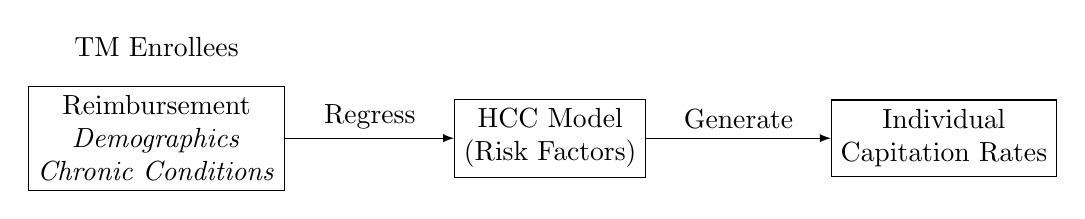
\begin{tikzpicture}
    \node[draw, rectangle, align=center] (input) at (0,0) { Reimbursement \\  \textit{Demographics}  \\  \textit{Chronic Conditions}};
    \node[above=0.25cm of input] {TM Enrollees};
    \node[draw, rectangle, align=center] (model) at (5,0) {HCC Model \\ (Risk Factors)};
    \node[draw, rectangle, align=center] (output) at (10,0) {Individual \\ Capitation Rates};
    
    \draw[->, >=latex] (input) -- (model) node[midway,above] {Regress};
    \draw[->, >=latex] (model) -- (output) node[midway,above] {Generate};
\end{tikzpicture}
    \caption{Capitation Rate Generation Process}
  \end{figure}
\end{frame}

\begin{frame}{Appendix: Risk Adjustment Outcomes}
  \begin{columns}
    \begin{column}{0.5\textwidth}
      \begin{figure}
        \centering
        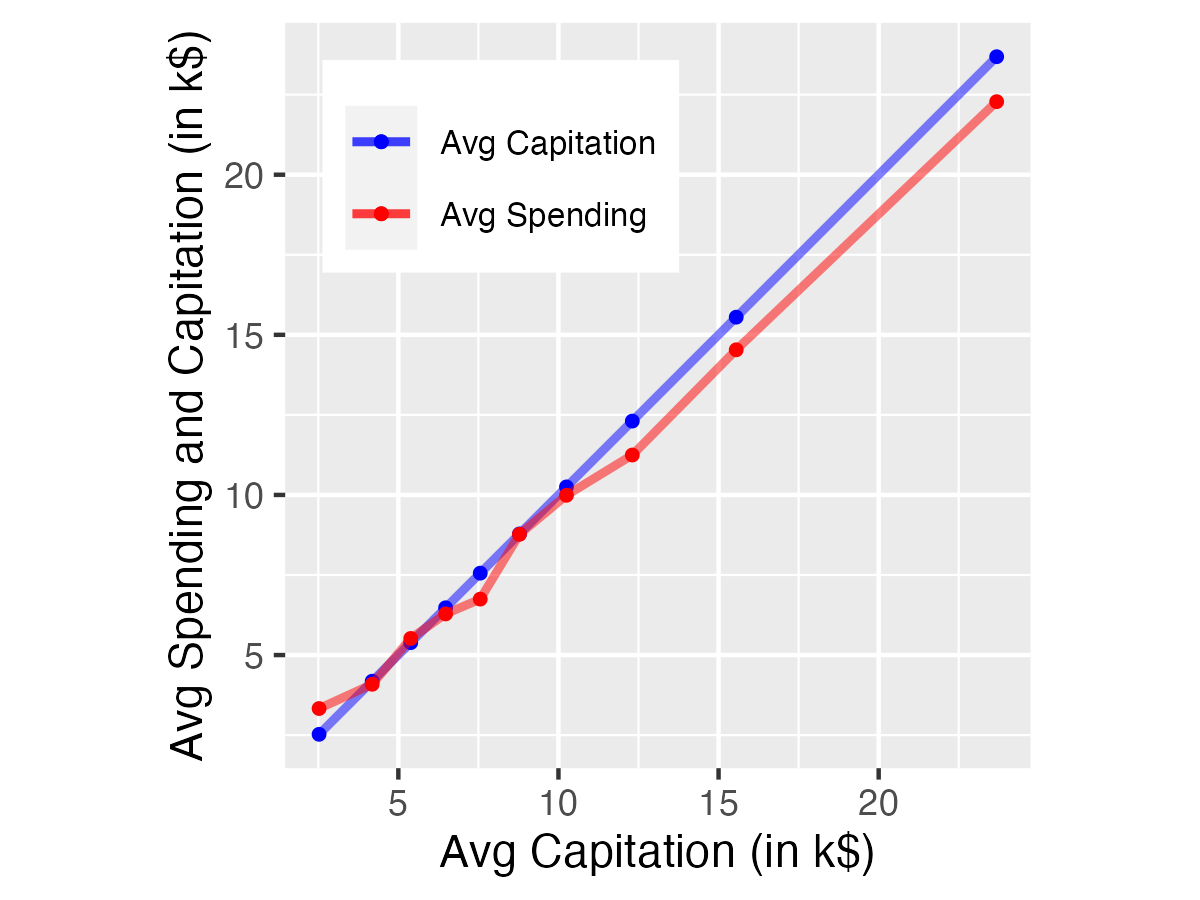
\includegraphics[width=1\textwidth]{figures/images/avg_spending_vs_capitation_by_capitation_deciles.png}
        \caption{Conditional on Capitation Deciles}
      \end{figure}
    \end{column}
    \begin{column}{0.5\textwidth}
      \begin{figure}
        \centering
        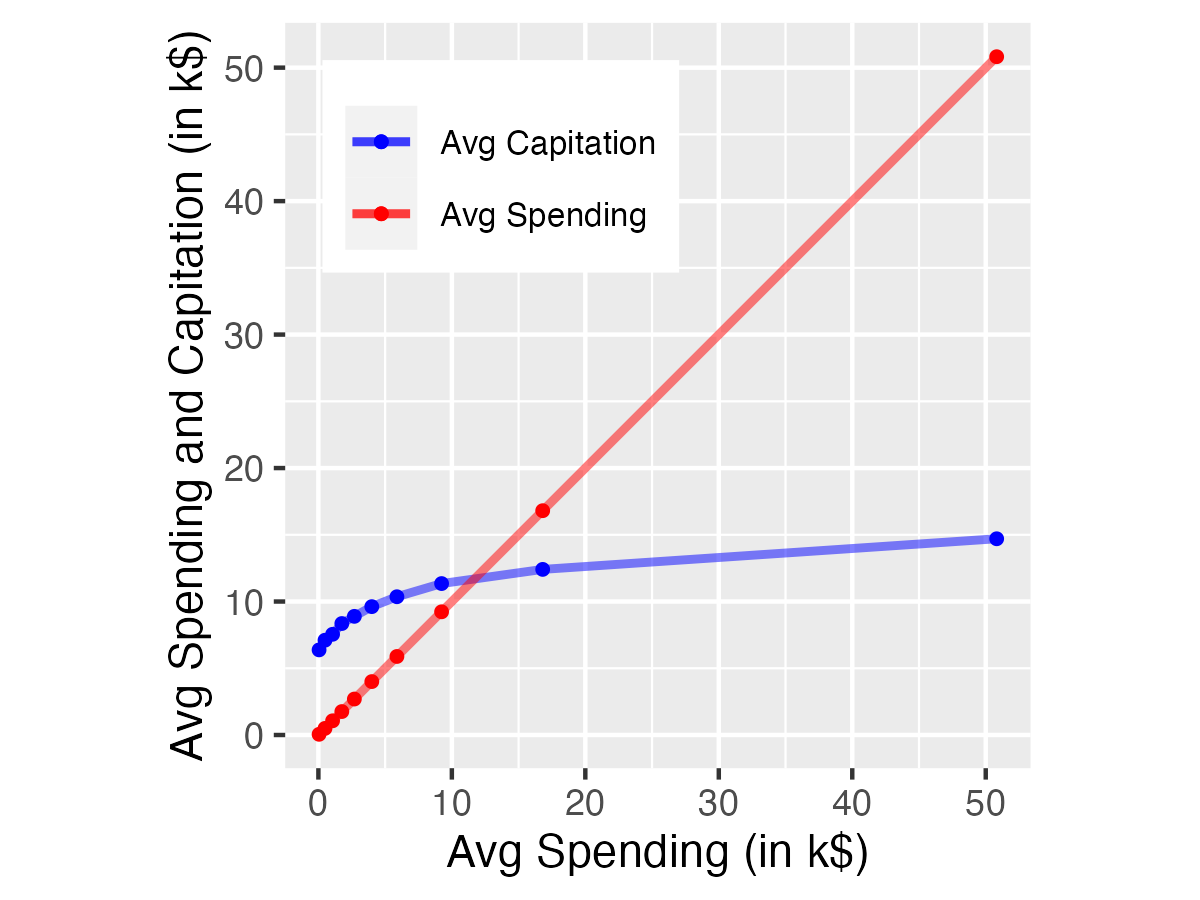
\includegraphics[width=1\textwidth]{figures/images/avg_spending_vs_capitation_by_spending_deciles.png}
        \caption{Conditional on Spending Deciles}
      \end{figure}
    \end{column}
    
  \end{columns}
\end{frame}

\begin{frame}{Appendix: Benefit Structure}
  \begin{figure}
    \begin{figure}
      \centering
      \resizebox{0.8\textwidth}{!}{\usetikzlibrary{positioning, fit, backgrounds}
\begin{tikzpicture}[
    block/.style={
      draw,
      rectangle,
      rounded corners,
      minimum height=2cm, 
      minimum width=3cm, 
      align=center
    },
    node distance=0.5cm
]
% Nodes of MA coverage
\node[block] (ma) {Medicare Basic\\Part A\&B Coverage};
\node[block, right=of ma] (supp) {MA\\Supplementary\\Part A\&B Coverage};
% make the add node in dashed line
\node[block, right=of supp, dashed] (add) {Additional Benefits \\ (e.g. Dental)};

% group the nodes
\begin{scope}[on background layer]
    % add title MA Benefits over the nodes
  \node[above=0.5cm of supp] {Medicare Advantage};
  \node[fit=(ma) (supp) (add), draw, inner sep=0.5cm] (ma_group) {};
\end{scope}

% add space between the two groups
\node[below=1cm of ma_group] {};

% Nodes of Medigap coverage
\node[block, below=2cm of ma] (medigap) {Medicare Basic\\Part A\&B Coverage};
\node[block, right=of medigap] (medigap_supp) {Medigap\\Supplementary\\Part A\&B Coverage};


% group the nodes
\begin{scope}[on background layer]
    % add title Medigap Benefits over the nodes
  \node[above=0.5cm of medigap_supp] {TM+Medigap};
  \node[fit=(medigap) (medigap_supp), draw, inner sep=0.5cm] (medigap_group) {};
\end{scope}

\end{tikzpicture}}
    \end{figure}
  \end{figure}
\end{frame}

\begin{frame}{An Example: Medicare Advantage}
  % insert the picture from figures/images/medicare_market.tex and center it
  \begin{figure}
    \centering
    \resizebox{0.6\textwidth}{!}{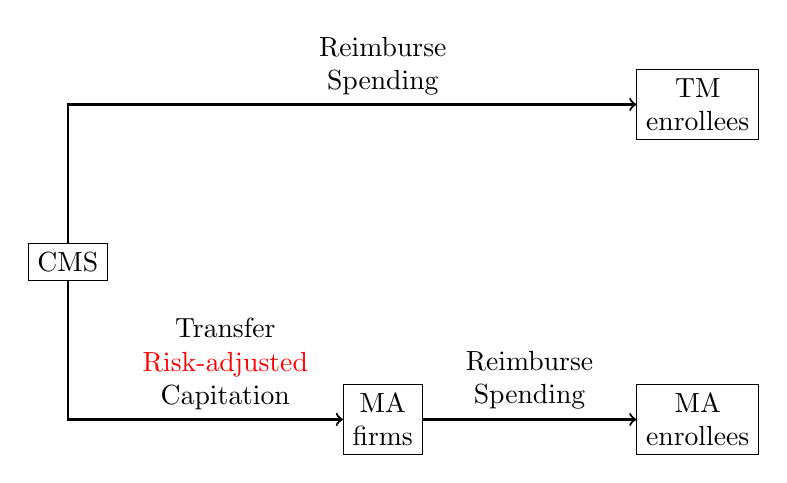
\begin{tikzpicture}
    \node[draw] (CMS) at (0,2) {CMS};
    \node[draw, align=center] (TM) at (8,4) {TM \\ enrollees};
    \node[draw, align=center] (MA) at (8,0) {MA \\ enrollees};
    \node[draw, align=center] (MAf) at (4,0) {MA \\ firms};

    \draw[->, thick] (CMS.north) |- (TM.west);
    \draw[->, thick] (CMS.south) |- (MAf.west);
    \draw[->, thick] (MAf.east) -- (MA.west) node[midway, above, align=center] {Reimburse \\ Spending};

    \node[above, align=center] at (4,4) {Reimburse \\ Spending};
    \node[above, align=center] at (2,0) {Transfer \\ \textcolor{red}{Risk-adjusted} \\ Capitation};
\end{tikzpicture}}
  \end{figure}
  \begin{itemize}\small
    \item Traditional Medicare (TM) is FFS.
    \item Medicare Advantage (MA) is managed competition.
    \item Beneficiaries choose between TM and MA.
  \end{itemize}
  \end{frame}
\end{document}